\begin{figure}[t]
\centering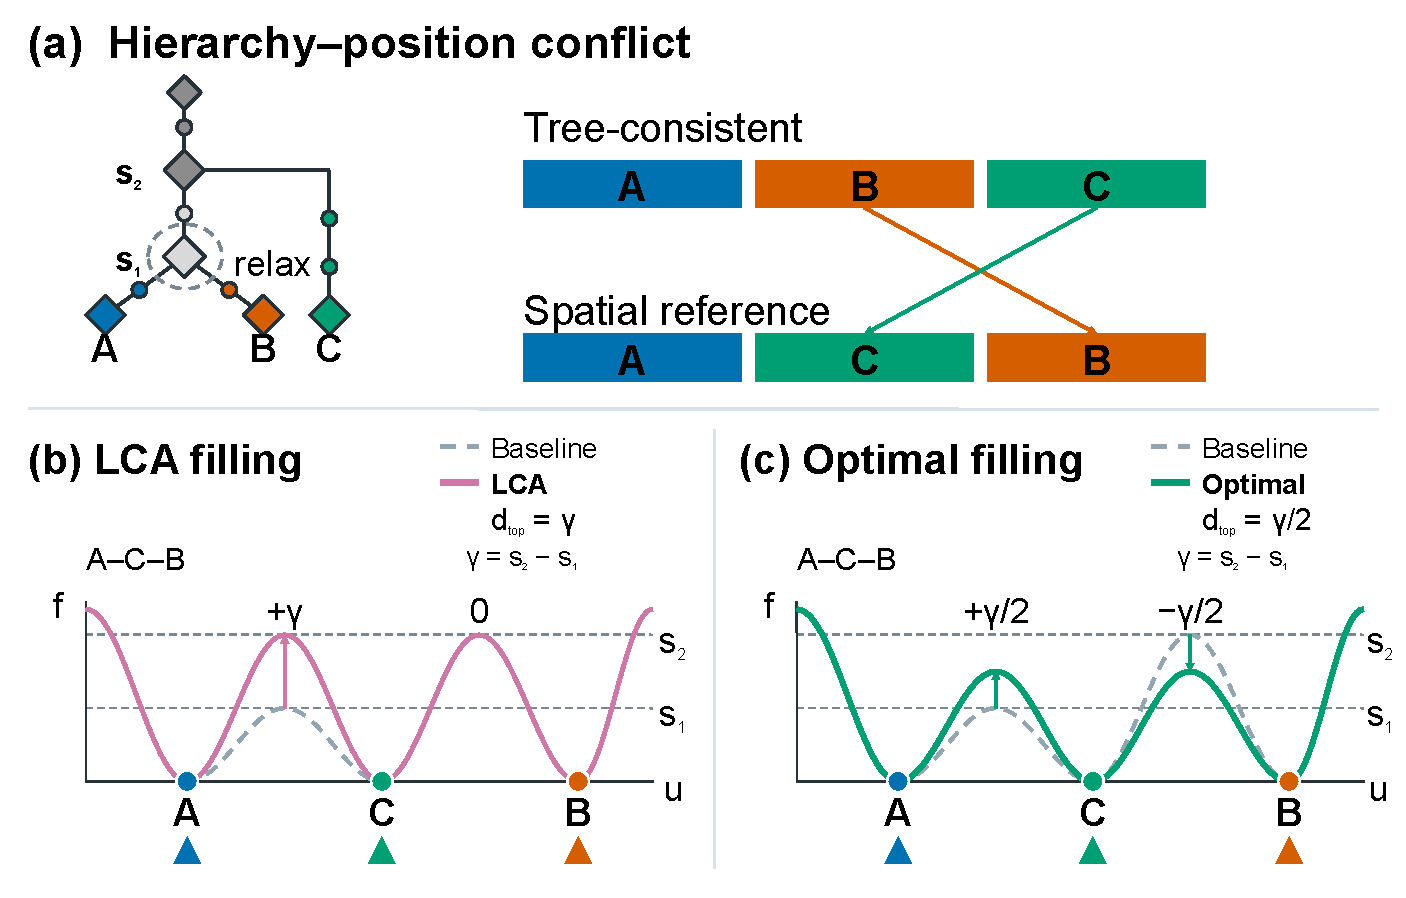
\includegraphics[width=\linewidth]{figures/Fig4.pdf}
\caption{Hierarchy--position conflict and scalar filling for three equal-valued minima. (a) The source tree groups $A,B$, excluding reference order $A,C,B$. Identity colours match the other schematics: $A$ blue, $B$ orange, and $C$ green. (b,c) Both fillings use the same relaxed anchors in order $A,C,B$, with identical reference triangles. Original-LCA filling (purple) sets both barriers to $s_2$, incurring $d_{\rm top}=\gamma=s_2-s_1$. Optimal filling (green) places both at $(s_1+s_2)/2$, attaining $\gamma/2$ when fixed leaf values lie below this level. The dashed grey baseline retains the hierarchy and its anchor displacement. Curves are schematic.}
\label{fig:filling}
\end{figure}
